\newpage
\section{Проведение эксперимента}
В данной работе источником излучения служит тлеющий разряд в воздухе.
Принципиальная схема регистрации излучения представлена на \figref{ust}. Излучение
регистрируется через боковую стенку разрядного отсека плазмотрона. Изображение плазмы в
масштабе 1:4 с помощью линзы из LiF фокусируется на входную щель монохроматора МДР-23.
\begin{figure}[H]
	\begin{center}
		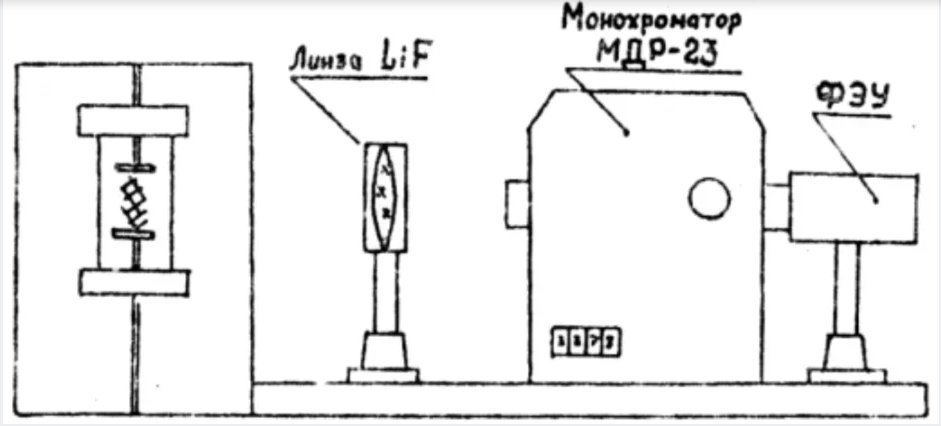
\includegraphics[width=0.99\textwidth]{ystanovka.png}
		\caption{Схема регистрации излучения}
		\label{ust}
	\end{center}	
\end{figure}

В качестве диспергирующего элемента монохроматора используется дифракционная
решетка, имеющая 1200 штрихов на миллиметр (1200 /1). За выходной щелью
монохроматора помешается фотоумножитель ФЭУ-100. Монохроматор МДР-23
используется в составе управляющего измерительного комплекса КСВУ-23, включающего
также ЭВМ ДВК-3, интерфейсные блоки связи ЭВМ с экспериментальной установкой,
усилитель с высокоомным входом, управляемый от ЭВМ источник высокого напряжения
для питания ФЭУ. Конструкция монохроматора позволяет осуществлять сканирование
спектра в автоматическом режиме с заданной скоростью. Дифракционная решетка при
этом поворачивается с помощью шагового двигателя.


Использование воздушной смеси азота и кислорода принципиально, так как при содержании кислорода менее 2 \% в спектре появляются полосы отрицательной ($1^{-}$)-системы ${N_2}^+$, чья интенивность может превосходить интенсивность (2+) системы.  